\documentclass[11pt,letterpaper]{article}
\usepackage[margin=1in]{geometry}
\usepackage{amsmath,booktabs,graphicx,hyperref,xurl}
\hypersetup{colorlinks=true,urlcolor=blue,linkcolor=blue}
\urlstyle{same}
\setlength{\parindent}{0pt}
\setlength{\parskip}{5pt}
\begin{document}
\hypersetup{pageanchor=false}
\begin{titlepage}
\centering
\vspace*{\fill}
{\LARGE\bfseries MORTIMER: Multi-asset Optimisation and Risk Targeting with Integrated Monthly E6 Rebalancing\par}
\vspace{2cm}
{\large Nelson Alvarez, Amir Hajomar, Sean Majewski, and Miles Rack\par}
\vspace{0.75cm}
{4 October 2026\par}
\vspace*{\fill}
\end{titlepage}
\hypersetup{pageanchor=true}
\newpage
\section*{Summary}
MORTIMER combines monthly equal-risk-contribution weights with a causal volatility overlay across six ETFs. On the held-out OOS test, the portfolio returned 9.52\% annualised after five basis points of trading costs, with 7.47\% volatility, a 0.714 Sharpe ratio, a $-7.00$\% maximum drawdown, and annual half-L1 turnover of 1.119. Relative to matched unscaled ERC, volatility fell by 8.2\% and drawdown by 9.9\%, while Sharpe also declined. Validation produced larger risk reductions at an annual return cost of 15 basis points. The evidence therefore indicates modest risk control, with no improvement in risk-adjusted return.

\section*{Economic hypothesis}
Investors accept equity, credit, duration, and commodity risk premia, while benchmark mandates and slow risk-budget adjustment can leave portfolios exposed as volatility rises. Since variance clusters, a forecast based on recent returns may help manage subsequent portfolio risk without predicting return direction. MORTIMER reduces risky exposure when forecast volatility exceeds its target. We test whether this rule lowers volatility and tail losses after costs, while limiting the associated return drag. A shock can arrive before the overlay responds, and lower exposure can delay recovery.

\section*{Data and universe}
The fixed universe comprises QQQ, IWM, HYG, TLT, GLD, and DBC. Yahoo adjusted closes include distributions and splits; raw closes and volume support liquidity estimates. Cash accrues from initial-release ALFRED DGS3MO observations, using the next exchange session for availability and ACT/365 between observations. The XNYS calendar spans 2 January 2008 to 2 October 2026, with 550 sessions reserved for estimation before scored returns. Training ends on 31 December 2018, and validation runs from 1 January 2019 to 1 October 2024. The competition rule reserves the shorter of the latest 20\% of sessions or two years; the resulting held-out OOS test runs from 2 October 2024 to 2 October 2026. Hashes and availability checks bind the inputs. The fixed surviving-fund universe and retrospectively adjusted prices limit historical representativeness.

\section*{Methodology}
At each month-end, estimate daily covariance from 126 completed observations using Ledoit--Wolf shrinkage toward a scaled-identity target (Ledoit and Wolf, 2004). The constrained equal-risk-contribution (ERC) allocation for six assets solves
\[
\min_b\sum_{i=1}^{6}\left[b_i(\widehat\Sigma_t b)_i-\frac{b^\top\widehat\Sigma_t b}{6}\right]^2,
\qquad \mathbf 1^\top b=1,\quad 0\le b_i\le0.35.
\]
Here $b_i$ is the base weight, $\widehat\Sigma_t$ is daily return covariance, and $b_i(\widehat\Sigma_t b)_i$ is variance contribution. Binding name caps can prevent exact equality.

For current base $b_t$, calculate historical portfolio returns $x_s=b_t^\top r_s$ using observations through close $t$. The annualised volatility forecast and capped risky exposure are
\[
\widehat\sigma_t=\sqrt{252\max\{\operatorname{EWMA}_{20}(x_s^2),\operatorname{EWMA}_{63}(x_s^2)\}},\qquad k_t=\min(1,0.10/\widehat\sigma_t).
\]
EWMA denotes an exponentially weighted moving average; each estimate requires 63 observations. Taking the larger estimate combines a faster response with a slower volatility measure. A five-percentage-point exposure change triggers a trade, while monthly base rebalances proceed independently. Gross exposure cannot exceed one, and the strategy neither shorts nor borrows. The 10\% forecast target does not fix realised volatility.

The close-$t$ signal is executed at close $t+1$, after that session's return; new holdings first earn the next close-to-close return. Given pre-fee risky holdings $h_i$, NAV $V$, desired weights $w_i$, and cost rate $c$, post-fee NAV satisfies
\[
V^{post}=V-c\sum_i|V^{post}w_i-h_i|.
\]
Costs are five basis points of risky dollars bought plus sold, representing spread, commission, and closing slippage; cash transfers carry no charge. The doubled-cost comparison uses ten basis points on development data. The single OOS record contains no doubled-cost run. DGS3MO is a cash-yield proxy, not a Treasury-bill total-return series.

\section*{Results}
CAGR compounds split-local net wealth using 252 sessions per year. Annual volatility is daily sample standard deviation times $\sqrt{252}$; Sharpe uses excess return over the causal cash proxy. Maximum drawdown includes initial wealth one. Turnover is annualised half the absolute change in risky and cash weights; transaction costs use risky purchases plus sales.
\input{../results/mortimer-submission/report-build/performance.tex}
\begin{center}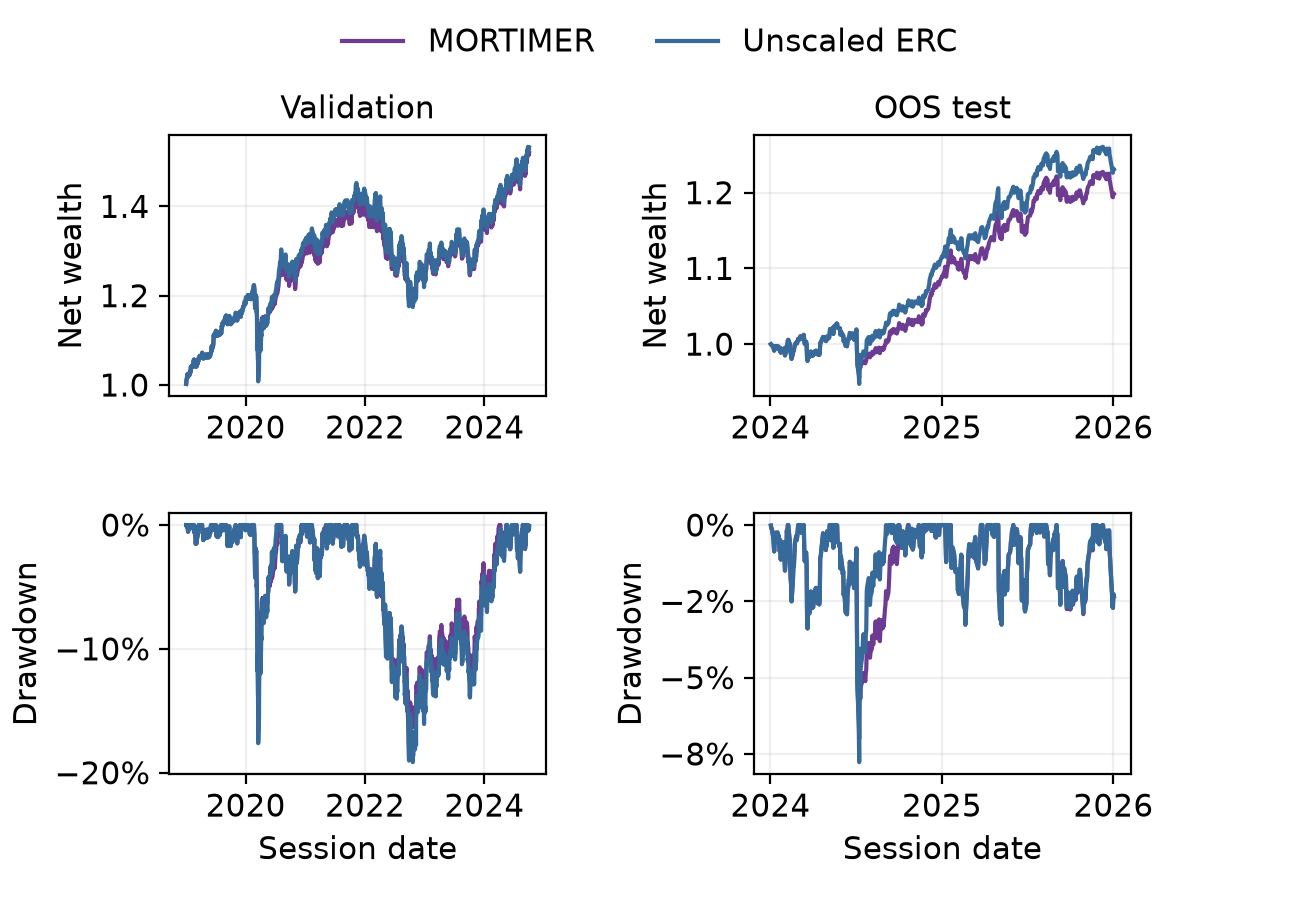
\includegraphics[width=0.80\linewidth]{split-evidence.png}\end{center}
\input{../results/mortimer-submission/report-build/result-discussion.tex}

The registered search comprised 12 primary configurations. OOS volatility and drawdown reductions fall below the 10\% thresholds, and Sharpe is below the matched unscaled portfolio.

\section*{Risk management}
Base weights are long-only and capped at 35\% per instrument. Gross exposure cannot exceed 100\%, with the remainder held as cash. Weights drift between executions and may exceed target caps. The overlay reduces or restores exposure when the forecast changes by five percentage points; it has no stop-loss or discretionary drawdown gate. Close-to-close execution leaves the portfolio exposed until the next order takes effect.

Forecast IC measures association with subsequent realised volatility, not return predictability; overlapping forward labels are dependent. The 2022 result and factor attribution describe adverse-regime performance and broad exposures.
\begin{center}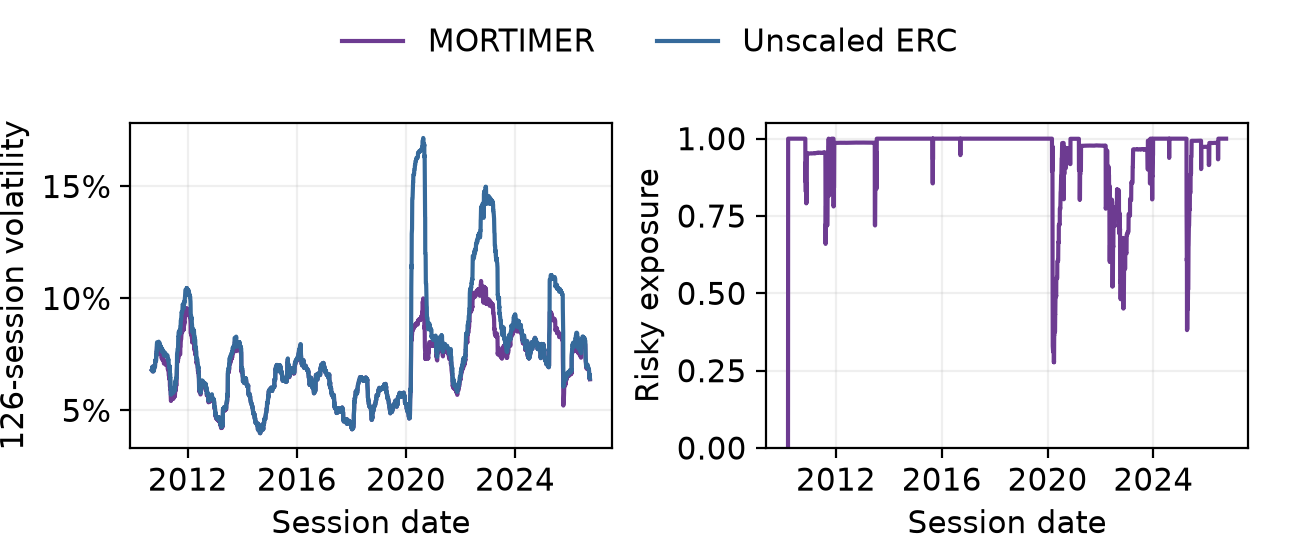
\includegraphics[width=0.78\linewidth]{risk-evidence.png}\end{center}
\input{../results/mortimer-submission/report-build/risk-discussion.tex}

\section*{Liquidity and capacity}
Liquidity is measured with previous-session trailing 20-session dollar average daily volume (ADV). Participation is $Q/ADV$, where $Q$ is risky trade notional. The square-root impact scenario is
\[
I=Y\sigma\sqrt{Q/ADV},\qquad \text{NAV cost}=I\,Q/NAV,
\]
We set $Y=0.5$ and use lagged volatility $\sigma$ for each AUM scenario.
\input{../results/mortimer-submission/report-build/capacity.tex}

\section*{Limitations and next steps}
MORTIMER lowers volatility and drawdown in validation, but the held-out reductions of 8.2\% and 9.9\% fall short of the registered thresholds; its OOS Sharpe is also below unscaled ERC. The observed benefit is therefore risk moderation rather than stronger risk-adjusted performance. Fixed surviving ETFs, retrospectively adjusted prices, a cash-yield proxy, closing-price execution, and a square-root impact approximation limit inference about implementation. A further study should use point-in-time fund histories and calibrated execution data under a separately registered evaluation.

\clearpage
\section*{References}
Andersen, T. G., Bollerslev, T., Diebold, F. X., and Labys, P. (2003). Modeling and forecasting realized volatility. \emph{Econometrica}, 71(2), 579--625. \url{https://doi.org/10.1111/1468-0262.00418}. Accessed 4 October 2026.

Bollerslev, T. (1986). Generalized autoregressive conditional heteroskedasticity. \emph{Journal of Econometrics}, 31(3), 307--327. \url{https://doi.org/10.1016/0304-4076(86)90063-1}. Accessed 4 October 2026.

Cont, R. (2001). Empirical properties of asset returns: stylized facts and statistical issues. \emph{Quantitative Finance}, 1(2), 223--236. \url{https://doi.org/10.1080/713665670}. Accessed 4 October 2026.

DeMiguel, V., Garlappi, L., and Uppal, R. (2009). Optimal versus naive diversification: how inefficient is the 1/N portfolio strategy? \emph{The Review of Financial Studies}, 22(5), 1915--1953. \url{https://doi.org/10.1093/rfs/hhm075}. Accessed 4 October 2026.

Engle, R. F. (1982). Autoregressive conditional heteroscedasticity with estimates of the variance of U.K. inflation. \emph{Econometrica}, 50(4), 987--1008. \url{https://doi.org/10.2307/1912773}. Accessed 4 October 2026.

Federal Reserve Bank of St. Louis (n.d.-a). \emph{DGS3MO: market yield on U.S. Treasury securities at three-month constant maturity}. FRED. \url{https://fred.stlouisfed.org/series/DGS3MO}. Accessed 4 October 2026.

Federal Reserve Bank of St. Louis (n.d.-b). \emph{Series observations}. FRED and ALFRED documentation. \url{https://fred.stlouisfed.org/docs/api/fred/series_observations.html}. Accessed 4 October 2026.

French, K. R. (n.d.). \emph{Data library}. Dartmouth College. \url{https://mba.tuck.dartmouth.edu/pages/faculty/ken.french/data_library.html}. Accessed 4 October 2026.

Ledoit, O. and Wolf, M. (2004). A well-conditioned estimator for large-dimensional covariance matrices. \emph{Journal of Multivariate Analysis}, 88(2), 365--411. \url{https://doi.org/10.1016/S0047-259X(03)00096-4}. Accessed 4 October 2026.

Maillard, S., Roncalli, T., and Teïletche, J. (2010). The properties of equally weighted risk contribution portfolios. \emph{The Journal of Portfolio Management}, 36(4), 60--70. \url{https://doi.org/10.3905/jpm.2010.36.4.060}. Accessed 4 October 2026.

Moreira, A. and Muir, T. (2017). Volatility-managed portfolios. \emph{The Journal of Finance}, 72(4), 1611--1644. \url{https://doi.org/10.1111/jofi.12513}. Accessed 4 October 2026.

Sharpe, W. F. (1994). The Sharpe ratio. \emph{The Journal of Portfolio Management}, 21(1), 49--58. \url{https://doi.org/10.3905/jpm.1994.409501}. Accessed 4 October 2026.

Tóth, B., Lempérière, Y., Deremble, C., de Lataillade, J., Kockelkoren, J., and Bouchaud, J.-P. (2011). Anomalous price impact and the critical nature of liquidity in financial markets. \emph{Physical Review X}, 1, 021006. \url{https://doi.org/10.1103/PhysRevX.1.021006}. Accessed 4 October 2026.

Yahoo Finance (n.d.). \emph{Historical market prices, adjustments, and volume}. Yahoo Finance. \url{https://finance.yahoo.com/}. Accessed 4 October 2026.

\end{document}
